\documentclass{article}
\usepackage{graphicx}
\usepackage{amsmath}
\usepackage{booktabs}
\usepackage{float}

\title{Malaria Transmission Dynamics with Mosquito Treatment: Reproduction Number Analysis}
\author{Yaghoub Shahmari}
\date{\today}

\begin{document}

\maketitle

\section{Model Description}
\subsection{Ordinary Differential Equations}
The model consists of 10 coupled ODEs tracking human and mosquito populations:

\textbf{Human Dynamics (SIS):}
\begin{align*}
    \frac{dS_H}{dt} &= -m a b (I_M + I_T) S_H + r I_H \\
    \frac{dI_H}{dt} &= m a b (I_M + I_T) S_H - r I_H
\end{align*}

\textbf{Untreated Mosquito Dynamics:}
\begin{align*}
    \frac{dS_M}{dt} &= g + h S_T - a c I_H S_M - t S_M - g S_M \\
    \frac{dE_{1,M}}{dt} &= a c I_H S_M - t E_{1,M} - s_{1M} E_{1,M} - g E_{1,M} \\
    \frac{dE_{2,M}}{dt} &= s_{1M} E_{1,M} - s_{2M} E_{2,M} - g E_{2,M} \\
    \frac{dI_M}{dt} &= s_{2M} E_{2,M} - g I_M
\end{align*}

\textbf{Treated Mosquito Dynamics:}
\begin{align*}
    \frac{dS_T}{dt} &= t S_M - a c I_H S_T - h S_T - g S_T \\
    \frac{dE_{1,T}}{dt} &= a c I_H S_T + t E_{1,M} - s_{1T} E_{1,T} - g E_{1,T} \\
    \frac{dE_{2,T}}{dt} &= s_{1T} E_{1,T} - s_{2T} E_{2,T} - g E_{2,T} \\
    \frac{dI_T}{dt} &= s_{2T} E_{2,T} - g I_T
\end{align*}

\subsection{Parameter Values}
Default parameter values used in simulations:

\begin{tabular}{lll}
    \toprule
    Parameter & Description & Default Value \\
    \midrule
    $a$ & Biting rate (day$^{-1}$) & 0.2 \\
    $b$ & Human-to-mosquito transmission probability & 0.5 \\
    $c$ & Mosquito-to-human transmission probability & 0.5 \\
    $m$ & Mosquito-to-human ratio & 20.0 \\
    $r$ & Human recovery rate (day$^{-1}$) & 0.01 \\
    $g$ & Mosquito death rate (day$^{-1}$) & 0.12 \\
    $h$ & Treatment waning rate (day$^{-1}$) & 0.1 \\
    $t$ & Treatment encounter rate (day$^{-1}$) & 0.1 \\
    $s_{1M}$ & Untreated $E_1 \rightarrow E_2$ rate (day$^{-1}$) & 0.2 \\
    $s_{2M}$ & Untreated $E_2 \rightarrow I$ rate (day$^{-1}$) & 0.2 \\
    $s_{1T}$ & Treated $E_1 \rightarrow E_2$ rate (day$^{-1}$) & 0.1 \\
    $s_{2T}$ & Treated $E_2 \rightarrow I$ rate (day$^{-1}$) & 0.1 \\
    \bottomrule
\end{tabular}

\begin{itemize}
    \item All rates expressed per day (day$^{-1}$)
    \item Human population normalized to 1 ($S_H + I_H = 1$)
    \item Mosquito populations tracked as proportions
\end{itemize}

\section{Methods}
\subsection{Reproduction Number Theory}
The basic ($R_0$) and effective ($R_{\text{eff}}$) reproduction numbers are calculated using the Next Generation Matrix (NGM). This approach linearizes the system around equilibrium points and quantifies infection spread potential.

\subsubsection{Disease-Free Equilibrium (DFE)}
The DFE is characterized by:
\begin{align*}
    I_H &= E_{1,M} = E_{2,M} = I_M = E_{1,T} = E_{2,T} = I_T = 0 \\
    S_H &= 1,\quad S_M = S_M^*,\quad S_T = S_T^*
\end{align*}
where $S_M^*$ and $S_T^*$ solve:
\begin{equation*}
    \begin{bmatrix}
        -(t + g) & h \\
        t & -(h + g)
    \end{bmatrix}
    \begin{bmatrix}
        S_M^* \\
        S_T^*
    \end{bmatrix}
    =
    \begin{bmatrix}
        -g \\
        0
    \end{bmatrix}
\end{equation*}

\subsubsection{Endemic Equilibrium (EE)}
The EE satisfies:
\begin{align*}
    \frac{dS_H}{dt} &= \frac{dI_H}{dt} = \cdots = \frac{dI_T}{dt} = 0 \\
    I_H &> 0,\quad I_M + I_T > 0
\end{align*}
Numerically found by solving the ODE system until convergence ($\|du/dt\| < 10^{-6}$).

\subsection{Next Generation Matrix Construction}
For infected compartments $\mathbf{x} = [I_H, E_{1,M}, E_{2,M}, I_M, E_{1,T}, E_{2,T}, I_T]^\top$:

\subsubsection{New Infections Matrix ($F$)}
\[
F = \begin{bmatrix}
0 & 0 & 0 & mabS_H^* & 0 & 0 & mabS_H^* \\
acS_M^* & 0 & 0 & 0 & 0 & 0 & 0 \\
0 & 0 & 0 & 0 & 0 & 0 & 0 \\
0 & 0 & 0 & 0 & 0 & 0 & 0 \\
acS_T^* & 0 & 0 & 0 & 0 & 0 & 0 \\
0 & 0 & 0 & 0 & 0 & 0 & 0 \\
0 & 0 & 0 & 0 & 0 & 0 & 0
\end{bmatrix}
\]
Where entries represent:
\begin{itemize}
    \item $F_{1,4}, F_{1,7}$: Mosquito-to-human transmission
    \item $F_{2,1}, F_{5,1}$: Human-to-mosquito transmission
\end{itemize}

\subsubsection{Transition Matrix ($V$)}
\[
V = \begin{bmatrix}
r & 0 & 0 & 0 & 0 & 0 & 0 \\
0 & t+s_{1M}+g & 0 & 0 & 0 & 0 & 0 \\
0 & -s_{1M} & s_{2M}+g & 0 & 0 & 0 & 0 \\
0 & 0 & -s_{2M} & g & 0 & 0 & 0 \\
0 & -t & 0 & 0 & s_{1T}+g & 0 & 0 \\
0 & 0 & 0 & 0 & -s_{1T} & s_{2T}+g & 0 \\
0 & 0 & 0 & 0 & 0 & -s_{2T} & g
\end{bmatrix}
\]
Key components:
\begin{itemize}
    \item Diagonal entries: Outflow from each compartment
    \item $V_{3,2}, V_{4,3}$: Untreated mosquito progression
    \item $V_{6,5}, V_{7,6}$: Treated mosquito progression
    \item $V_{5,2}$: Treatment transition $E_{1,M} \rightarrow E_{1,T}$
\end{itemize}

\subsection{Reproduction Number Calculation}
\subsubsection{Basic Reproduction Number ($R_0$)}
\[
R_0 = \rho(FV^{-1}) \quad \text{at DFE}
\]
where $\rho$ denotes spectral radius. This represents expected secondary infections in a fully susceptible population.

\subsubsection{Effective Reproduction Number ($R_{\text{eff}}$)}
\[
R_{\text{eff}} = \rho(\tilde{F}\tilde{V}^{-1}) \quad \text{at EE}
\]
where $\tilde{F}$ and $\tilde{V}$ use equilibrium values:
\begin{itemize}
    \item $S_H^{\text{EE}} < 1$, $S_M^{\text{EE}} < S_M^*$, $S_T^{\text{EE}} < S_T^*$
    \item Maintains same matrix structure as $F$ and $V$
\end{itemize}

\subsection{Numerical Implementation}
\begin{itemize}
    \item Matrix inversion via LU decomposition
    \item Eigenvalue calculation using QR algorithm
    \item DFE validation: $\|S_H + I_H - 1\| < 10^{-8}$
    \item EE convergence: Slope $<10^{-6}$ over 50 iterations
\end{itemize}

\section{Results}
\subsection{Model Dynamics}
\begin{figure}[H]
    \centering
    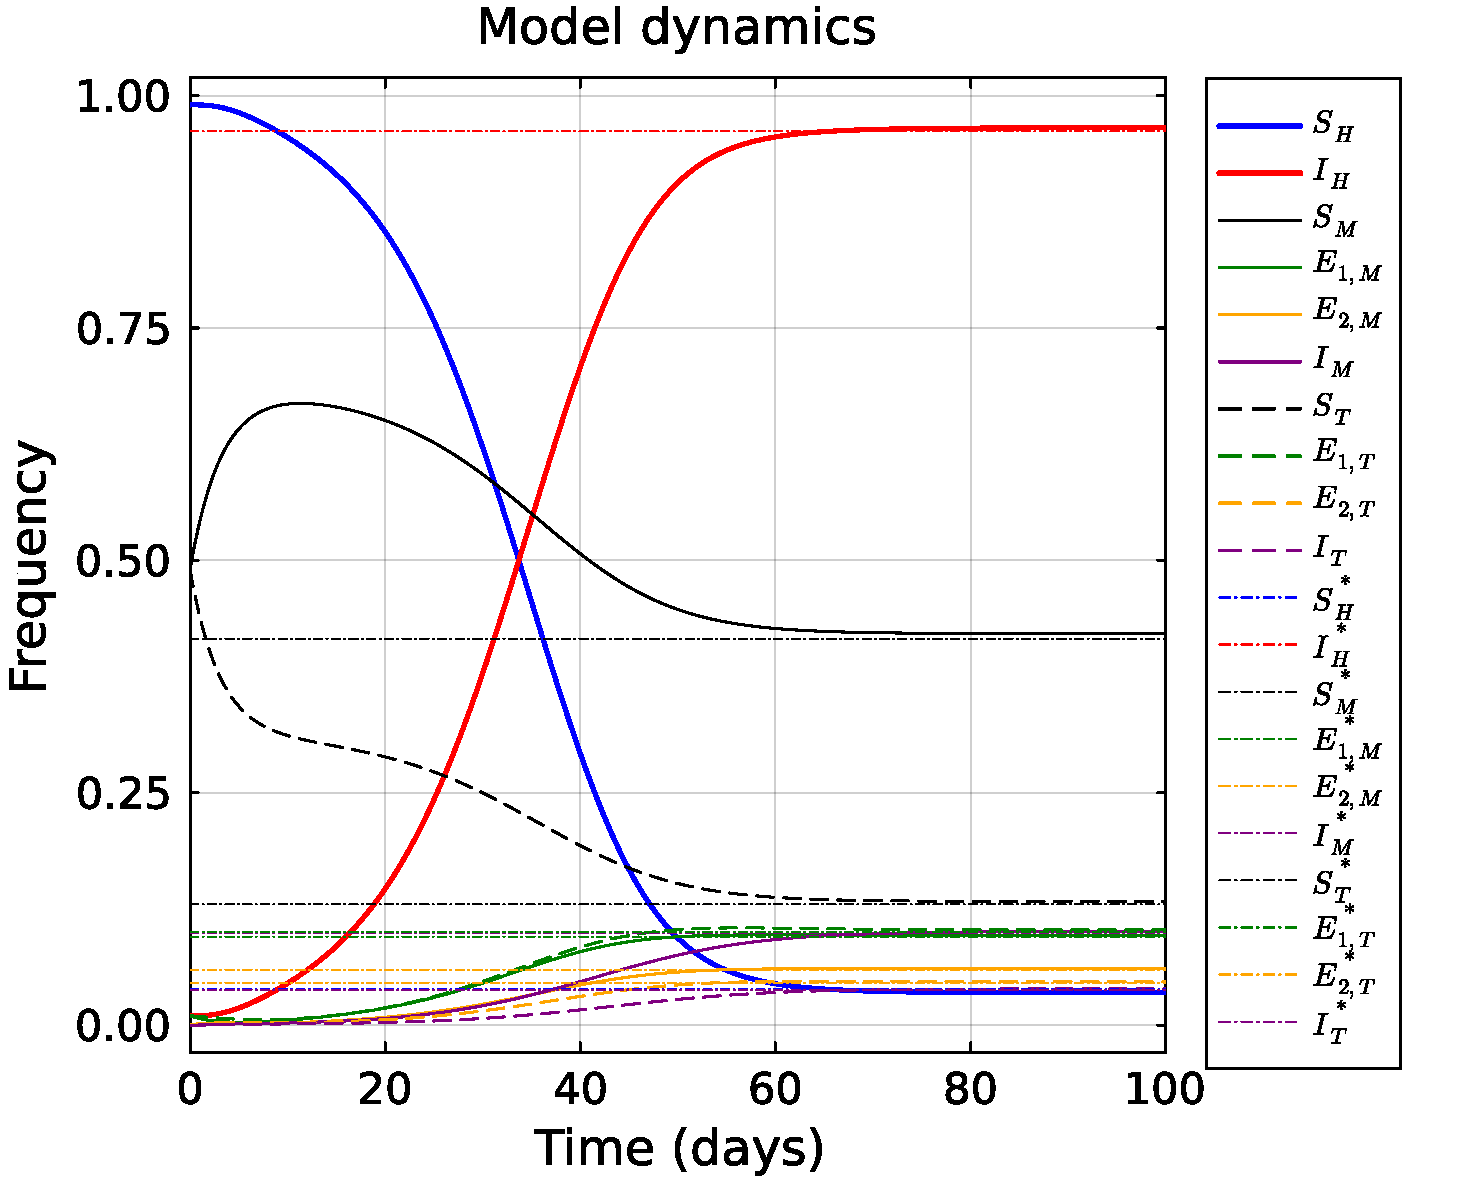
\includegraphics[width=0.49\textwidth]{../../fig/model_dynamics.pdf}
    \caption{Convergence to endemic equilibrium with default parameters: $R_0\approx7.1$, $R_{eff}\approx1.00005$.}
\end{figure}

\subsection{Basic Reproduction Number Analysis}
\begin{figure}[H]
    \centering
    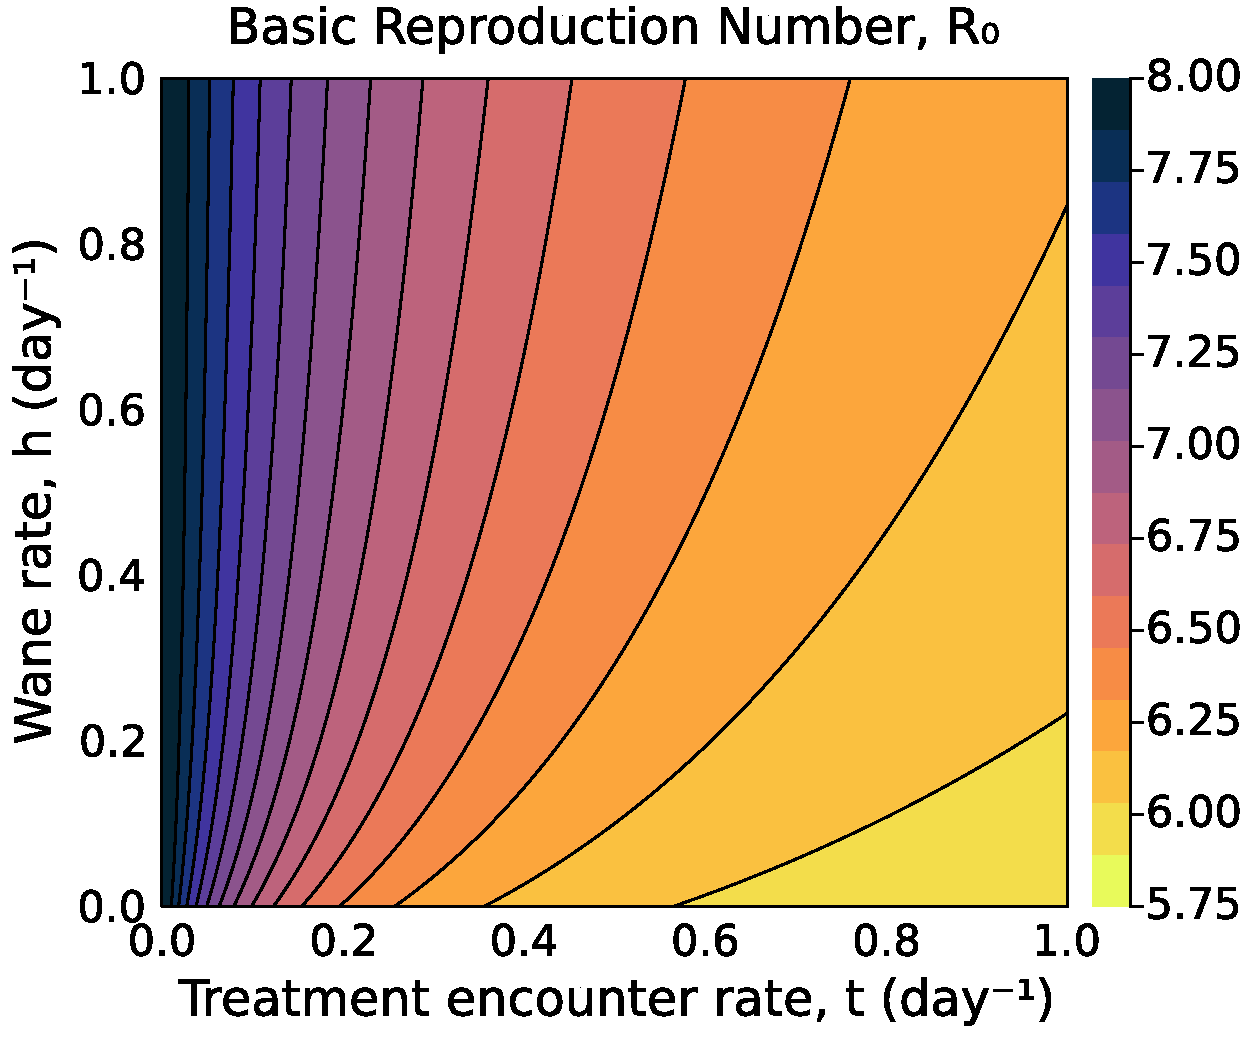
\includegraphics[width=0.49\textwidth]{../../fig/brn_txh_heatmap.pdf}
    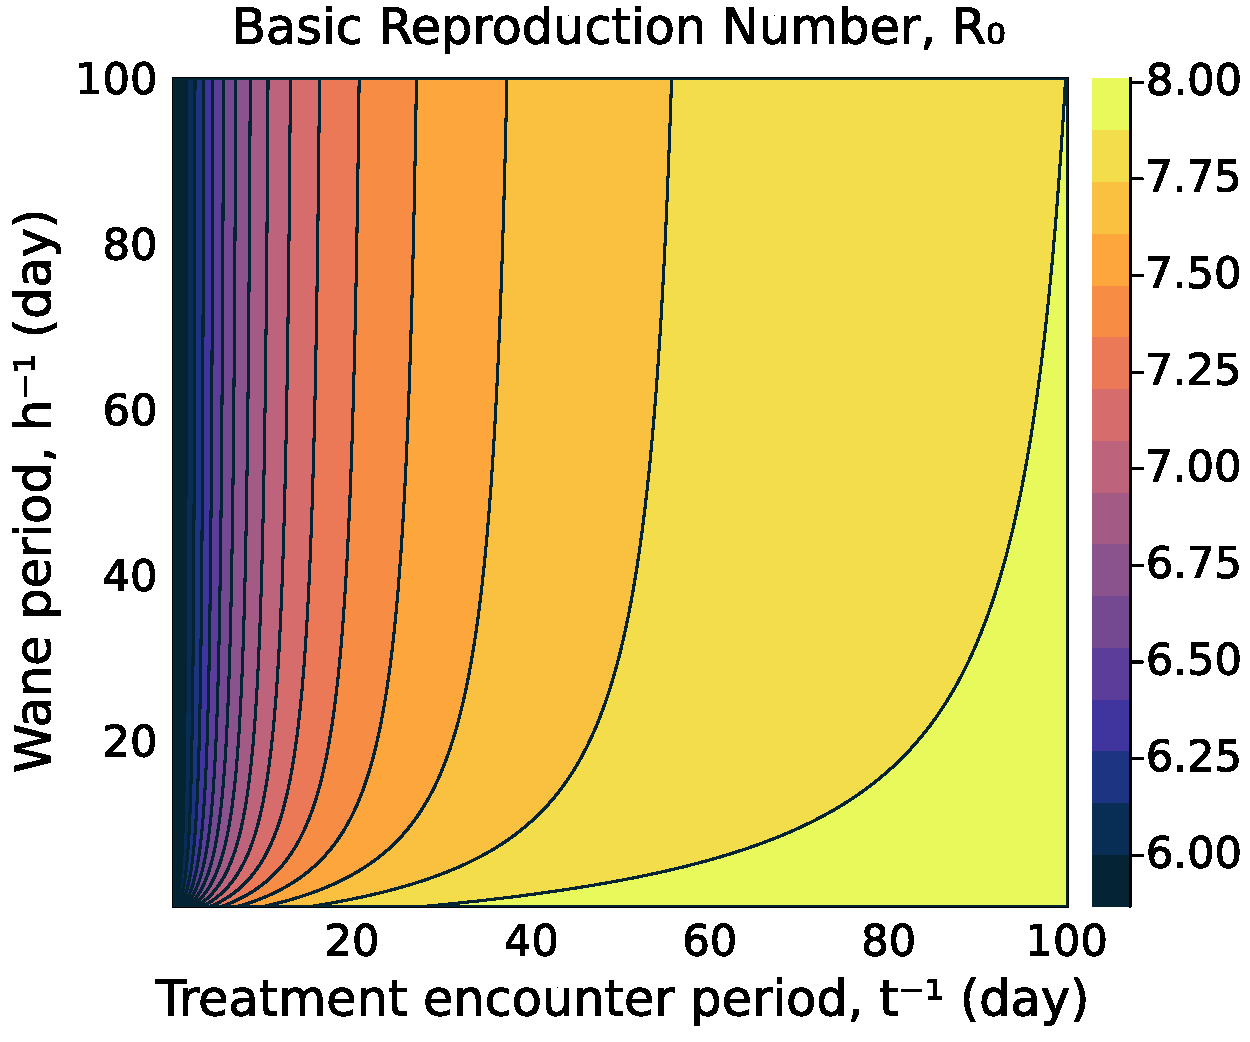
\includegraphics[width=0.49\textwidth]{../../fig/brn_txh_heatmap_rev.pdf}
    \caption{$R_0$ vs treatment rates ($t,h$) and treatment periods ($1/t,1/h$).}
\end{figure}

\subsection{Effective Reproduction Number}
\begin{figure}[H]
    \centering
    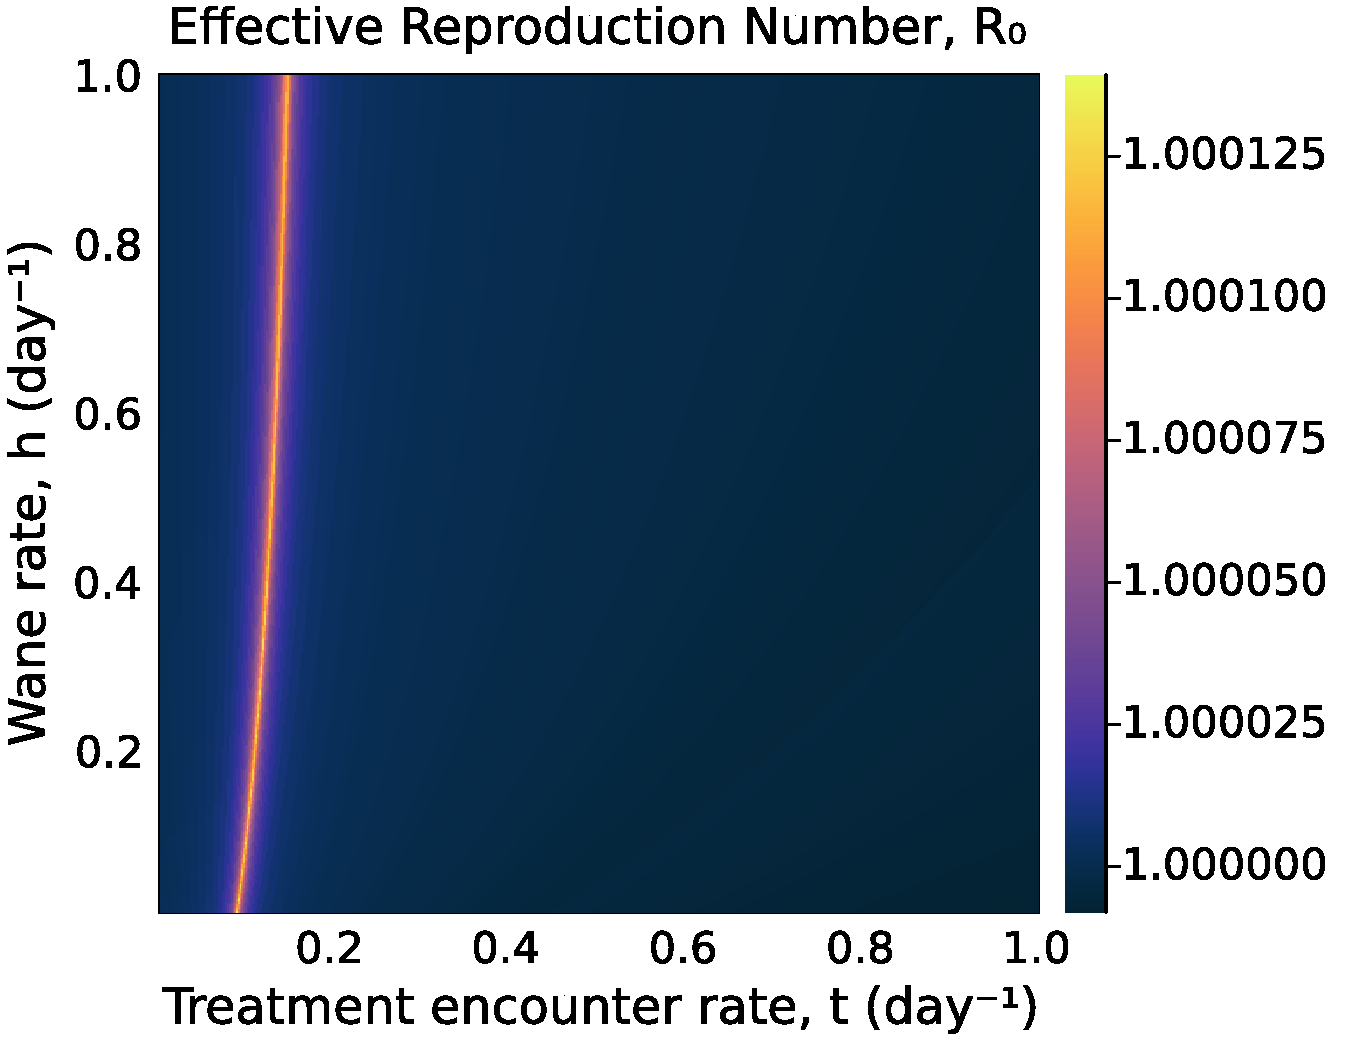
\includegraphics[width=0.49\textwidth]{../../fig/ern_txh_heatmap.pdf}
    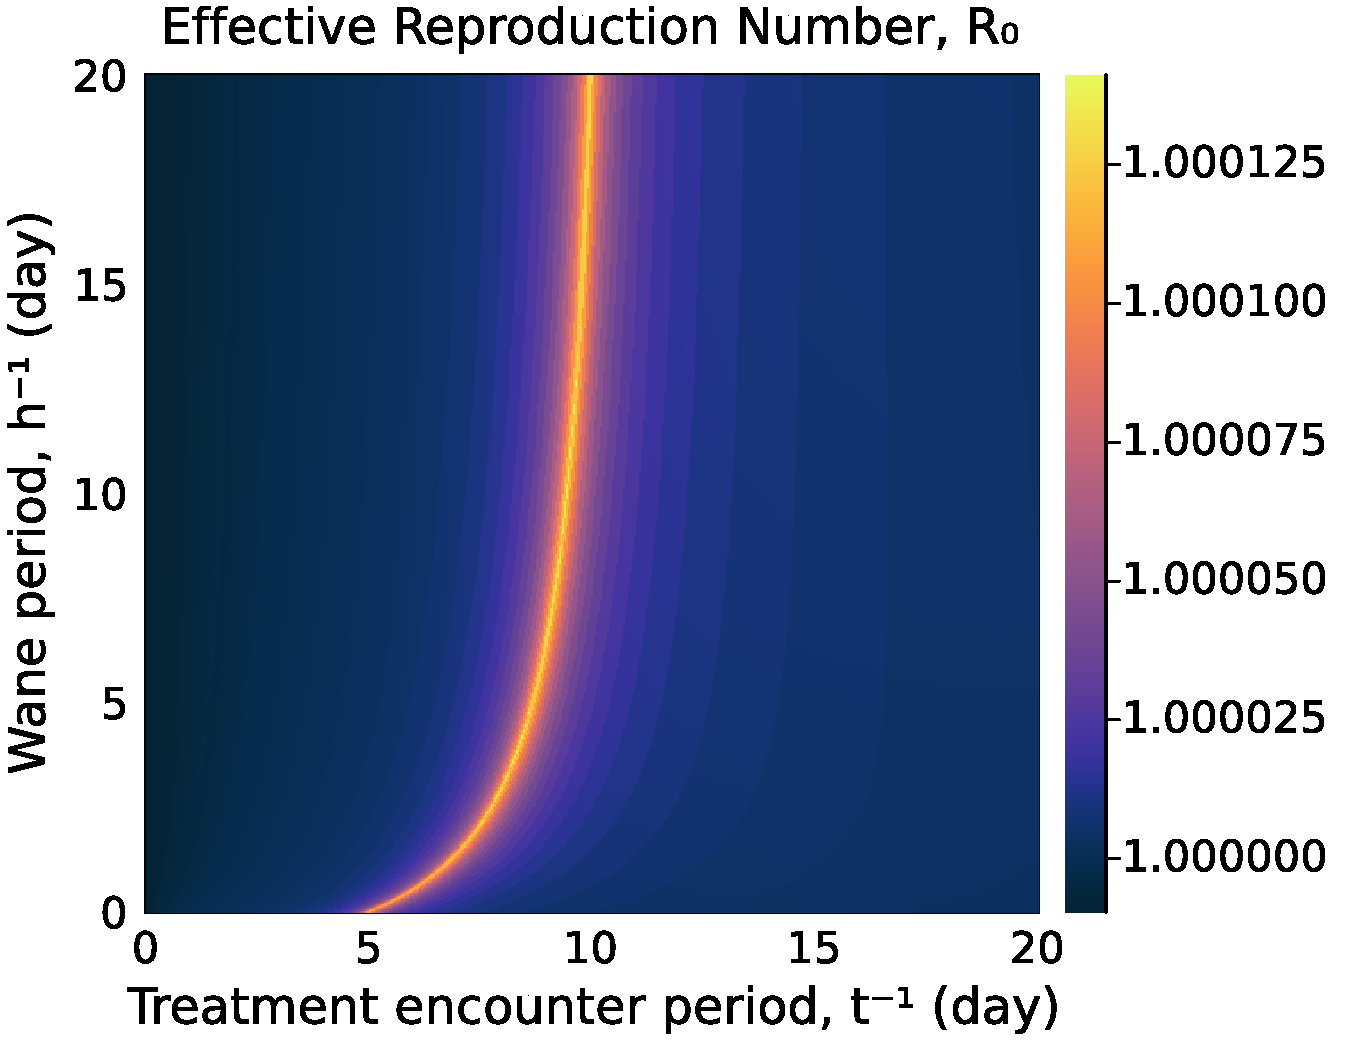
\includegraphics[width=0.49\textwidth]{../../fig/ern_txh_heatmap_rev.pdf}
    \caption{$R_{eff}$ vs treatment rates ($t,h$) and treatment periods ($1/t,1/h$).}
\end{figure}

\end{document}